\section{Análisis de Correspondencias}

\begin{itemize}
    \item Se realiza sobre variables categóricas. Se quiere estudiar relaciones entre las variables y las categorías de las mismas.
    \item Test $\chi^2$ de independencia: \[H_0:p_{ij}=p_{i+}\times p_{+j}, \quad \forall i=1,\dots,r,j=1;\dots,c\] donde \[\chi^2 = \sum_{i=1}^{r}\sum_{j=1}^{c}\frac{(n_{ij}-\frac{n_{i+}n_{+j}}{n_{++}})^2}{\frac{n_{i+}n_{+j}}{n_{++}}}=\sum_{i=1}^{r}\sum_{j=1}^{c}\frac{(Obs_{ij}-Esp_{ij})^2}{Esp_{ij}}\thicksim \chi^2_{(r-1),(c-1)}\]
    \item Perfiles fila y columna: Son las distribuciones condicionadas por filas y columnas. \[\text{Perfiles Fila: }\begin{pmatrix}\frac{n_{i1}}{n_{i+}}, & \cdots, & \frac{n_{ic}}{n_{i+}}\end{pmatrix}, \quad \forall i=1,\dots,r\] \[\text{Perfiles Columna: }\begin{pmatrix}\frac{n_{1j}}{n_{+j}}, & \cdots, & \frac{n_{rj}}{n_{+j}}\end{pmatrix}', \quad \forall j=1,\dots,c\]
    \item Si consideramos las frecuencias relativas $f_{ij}=\frac{n_{ij}}{n_{++}}$, $f_{i+}=\frac{n_{i+}}{n_{++}}$ y $f_{+j}=\frac{n_{+j}}{n_{++}}$ entonces: \[\text{Perfiles Fila: }\begin{pmatrix}\frac{f_{i1}}{f_{i+}}, & \cdots, & \frac{f_{ic}}{f_{i+}}\end{pmatrix}, \quad \forall i=1,\dots,r\] \[\text{Perfiles Columna: }\begin{pmatrix}\frac{f_{1j}}{f_{+j}}, & \cdots, & \frac{f_{rj}}{f_{+j}}\end{pmatrix}', \quad \forall j=1,\dots,c\]
    \item Centros de Gravedad de las nubes: \[\text{Para los perfiles fila: }\begin{pmatrix}f_{+1}, & \cdots, & f_{+r}\end{pmatrix}\] \[\text{Para los perfiles columna: }\begin{pmatrix}f_{1+}, & \cdots, & f_{c+}\end{pmatrix}\]
    \item Distancia $\chi^2$: Se utiliza para medir las distancias entre perfiles. \[\text{Distancia entre perfiles fila: }d^2_{\chi^2}(i,i')=\sum_{j=1}^{c}\frac{1}{f_{+j}}(\frac{f_{ij}}{f_{i+}}-\frac{f_{i'j}}{f_{i'+}})^2\] \[\text{Distancia entre perfiles columna: }d^2_{\chi^2}(j,j')=\sum_{i=1}^{c}\frac{1}{f_{i+}}(\frac{f_{ij}}{f_{+j}}-\frac{f_{ij'}}{f_{+j'}})^2\]
    \item Inercia Total: La inercia total define como $I_t=\sum_{i=1}^{r}\text{peso}(\text{fila}_i)d^2_{\chi^2}(\text{fila}_i,G_{\text{filas}})$ o también $I_t=\sum_{j=1}^{c}\text{peso}(\text{columna}_j)d^2_{\chi^2}(\text{columna}_j,G_{\text{columnas}})$
    \item $I_t=\frac{\chi^2}{n_{++}}$
    \item $F_{(r\times c)}=(f_{ij})$ matriz de las frecuencias relativas.
    \item $D_c=diag(f_{+1},\dots,f_{+c})$ y $D_r=diag(f_{1+},\dots,f_{r+})$ matrices diagonales que contienen las distribuciones marginales.
    \item Distancia entre perfiles fila: \[d^2_{\chi^2}(x,y)=(x-y)'D_c^{-1}(x-y)\] Distancia entre perfiles columna: \[d^2_{\chi^2}(x,y)=(x-y)'D_r^{-1}(x-y)\]
    \item $A=D_c^{-1}F'D_r^{-1}FD_c^{-1}$
    \item Para los perfiles fila, el vector $u$ que maximiza la inercia explicada es el autovector correspondiente al mayor autovalor de $D_cA=F'D_r^{-1}FD_c^{-1}$.
    \item Para los perfiles columna, el vector $u$ que maximiza la inercia explicada es el autovector correspondiente al mayor autovalor de $FD_c^{-1}F'D_r^{-1}$.
    \item Los autovalores asociados a las matrices correspondientes a los perfiles fila y columna son los mismos.
    \item En perfiles fila denominaremos:
          \begin{itemize}
              \item Eje principal $\alpha$, $u_\alpha$, al autovector asociado al autovalor $\lambda_\alpha$.
              \item Factor $\alpha$, $\varphi_\alpha=D_c^{-1}u_\alpha$
              \item Las proyecciones sobre el eje principal $u_\alpha$; se calculan como $\hat{u}_\alpha=(D_r^{-1}F)\varphi_\alpha$.
          \end{itemize}
          En perfiles columna denominaremos:
          \begin{itemize}
              \item Eje principal $\alpha$, $v_\alpha$, al autovector asociado al autovalor $\lambda_\alpha$.
              \item Factor $\alpha$, $\psi_\alpha=D_r^{-1}v_\alpha$
              \item Las proyecciones sobre el eje principal $v_\alpha$; se calculan como $\hat{v}_\alpha=(D_c^{-1}F')\psi_\alpha$.
          \end{itemize}
    \item Relaciones de transición: \[v_\alpha=\frac{1}{\lambda_\alpha}FD_c^{-1}u_\alpha \quad \psi_\alpha=\frac{1}{\lambda_\alpha}D_r^{-1}F\varphi_\alpha\] Reciprocramente tenemos \[u_\alpha=\frac{1}{\lambda_\alpha}F'D_r^{-1}v_\alpha \quad \varphi_\alpha=\frac{1}{\lambda_\alpha}D_c^{-1}F'\psi_\alpha\]
    \item Las proyecciones sobre el autovector vector fila/columna promedio son siempre $\overline{1}$.
    \item Contribuciones absolutas (a la inercia explicada por cada eje): Del perfil fila $i$ al eje $\alpha$ \[c.a.(i,\alpha)=f_{i+}\psi^2_{\alpha i}\] Del perfil columna $j$ al eje $\alpha$ \[c.a.(j,\alpha)=f_{+j}\varphi^2_{\alpha i}\]
    \item Contribuciones relativas (cosenos cuadrados): Del perfil fila $i$ al eje $\alpha$ \[c.r.(i,\alpha)=\frac{\hat{\psi}^2_{\alpha i}}{\sum_{\alpha}\hat{\psi}^2_{\alpha i}}\] Del perfil columna $j$ al eje $\alpha$ \[c.r.(j,\alpha)=\frac{\hat{\varphi}^2_{\alpha j}}{\sum_{\alpha}\hat{\varphi}^2_{\alpha j}}\]
    \item Mismos criterios de interpretación de resultados que en el ACP.
    \item Al escoger el número de dimensiones a extraer, la reprentación perfecta de las distancias será en $T=min(r-1, c-1)$ dimensiones.
    \begin{itemize}
        \item Aún así, lo más habitual es retener las dos primeras dimensiones, para hacerse la mejor idea a partir de una representación bidimensional.
        \item También se puede tener en cuenta como criterio el porcentaje de inercia a retener.
        \item O gráficamente, representando un scree plot y encontrando el ``codo''.
    \end{itemize}
    \item \textbf{Gráficos asimétricos:} Se representa uno de los grupos de perfiles (el que tenga más interés) mediante las coordenadas obtenidas en el análisis y el otro grupo se representa a través de las coordenadas estandares (proyecciones de los vértices del simplejo)
    \begin{figure}[ht]
        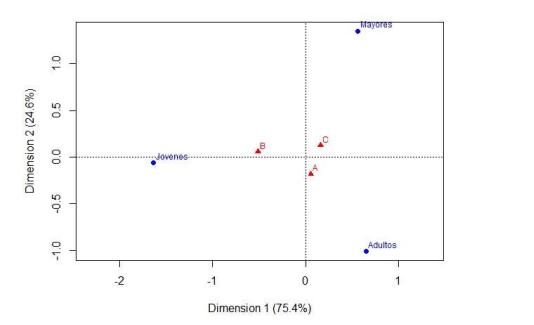
\includegraphics[width=\textwidth]{assets/grafico_asimetrico.png}
    \end{figure}
    
    \newpage

    \item \textbf{Mapas simétricos:} Son los más habituales. En esta ocasión tanto las filas como las columnas se representan en sus coordenadas principales (las obtenidas del análisis). No se pueden interpretar las distancias entre perfiles filas y columnas, ya que originalmente son espacios distintos e incluso podrían tener diferente dimensión.
    \item Se puede pasar del gráfico asimétrico al simétrico realizando una ``contracción'' igual a la raiz cuadrada del autovalor correspondiente a cada eje (no entendi nada xd).
    \begin{figure}[ht]
        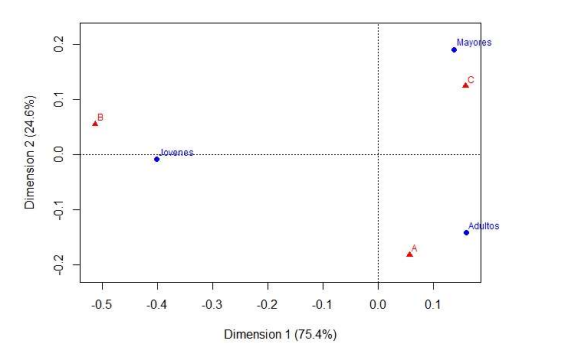
\includegraphics[width=\textwidth]{assets/grafico_simetrico.png}
    \end{figure}
    
    Vemos que a pesar de parecer ``cercanos'' Jovenes y el producto B, al no poder sacar conclusiones, sería injustificado decir que \textit{los jovenes prefieren el producto B}, y además, en este ejemplo, falso.
    \item \textbf{Biplots:} Solo se representa uno de los conjuntos en coordenadas principales. Los mapas asimétricos son un ejemplo de biplot, pero hay más tipos, como el biplot estandar.
    \begin{figure}[ht]
        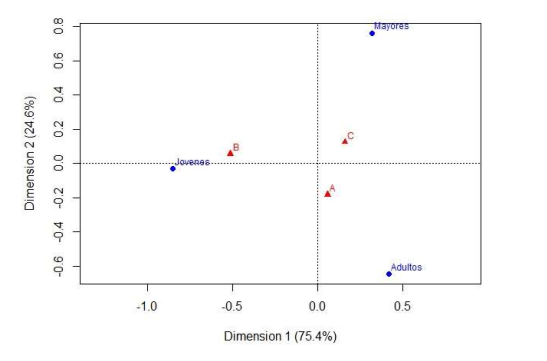
\includegraphics[width=\textwidth]{assets/grafico_biplot.png}
    \end{figure}
    \item No pueden interpretarse las distancias entre los puntos no representados en coordenadas principales, pero estos indican las direcciones de los ejes del biplot, y las coordenadas principales representadas sobre estos ejes si que son indicativas de la distancia entre esos puntos y la clase correspondiente a ese vértice.

    \newpage

    \item En la práctica aparecen casos típicos, los más comunes son los siguientes:
    \begin{itemize}
        \item Existencia de una asociación entre grupos de clases de las filas y grupos de clases de las columnas. Esto genera una representación en la que aparecen nubes de puntos separadas entre si donde están agrupadas las clases de fila y columna entre las que existe dicha asociación.
        \begin{figure}[ht]
            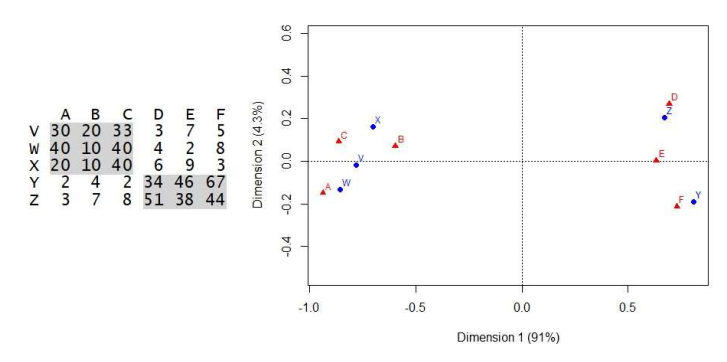
\includegraphics[width=\textwidth]{assets/asociacion_gruopos1.png}
        \end{figure}
        \begin{figure}[ht]
            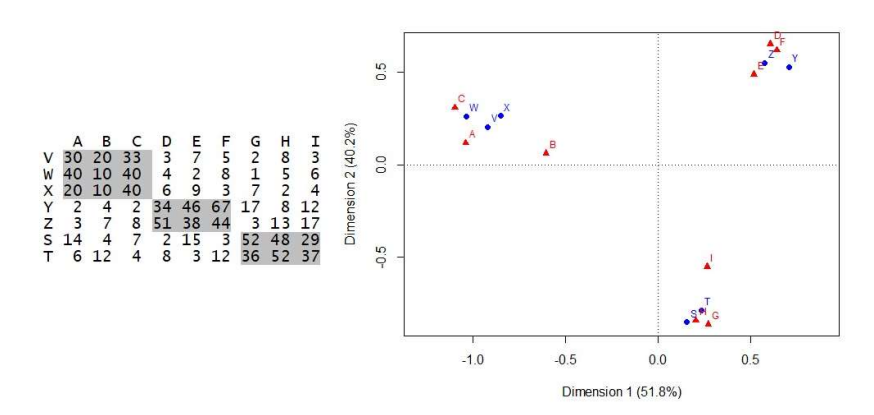
\includegraphics[width=\textwidth]{assets/asociacion_gruopos2.png}
        \end{figure}
        \newpage
        \item Existencia de una asociación fuerte entre dos variables categóricas que se analizan. De modo que los valores altos de la tabla de contingencia aparecen en la diagonal, y los puntos en los gráficos sigen el ``Efecto Guttman'' formando una nube con forma de parabola.
        \begin{figure}[ht]
            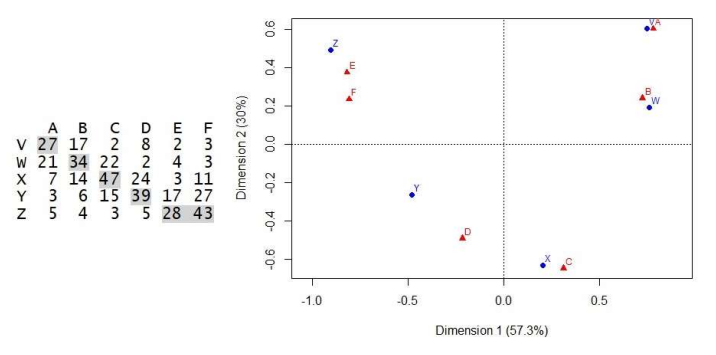
\includegraphics[width=\textwidth]{assets/asociacion_guttman.png}
        \end{figure}
        \newpage
        \item Existencia de una relación circular. Se relacionan en el mismo sentido valores altos y bajos.
        \begin{figure}[ht]
            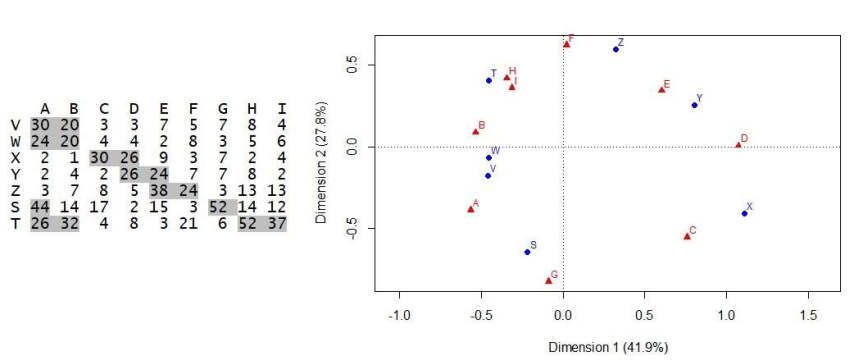
\includegraphics[width=\textwidth]{assets/asociacion_circular.png}
        \end{figure}
    \end{itemize}
    \item Se pueden añadir, igual que en ACP, elementos suplementarios (columnas o filas). Los elementos suplementarios corresponen a observaciones posteriores, en condiciones distintas, de naturaleza distinta\dots.
    \item Se proyectan en el análisis y se interpretan por proximidad a los elementos activos.
    \item No tienen contribuciones absolutas pero si relativas.
    \item Para hacer las proyecciones se utilizan las relaciones de transición o los factores.
    \item Proyecciones de elemntos suplementarios sobre el eje alpha:
    \[
        \text{Columna suplementaria:} \quad \hat{\varphi}^{+}_\alpha=\frac{1}{\sqrt{\lambda_\alpha}}\sum_{i=1}^r\left(\frac{n^{+}_i}{n^{+}_{+}}\right)\hat{\psi}_{\alpha i}=\sum_{i=1}^r\left(\frac{n^{+}_{i}}{n^{+}_{+}}\right)\psi_{\alpha i}
    \]
    \[
        \text{Fila suplementaria:} \qquad\quad \hat{\psi}^{+}_\alpha=\frac{1}{\sqrt{\lambda_\alpha}}\sum_{j=1}^c\left(\frac{n^{+}_j}{n^{+}_{+}}\right)\hat{\varphi}_{\alpha j}=\sum_{j=1}^c\left(\frac{n^{+}_{j}}{n^{+}_{+}}\right)\varphi_{\alpha j}
    \]
    \item Una de las aplicaciones del AC es asignar valores numéricos a las categorías de las variables implicadas.
    \item Sean $z_c(1),\dots,z_c(c)$ los valores numéricos a asignar a las $c$ categorías de una variable e $Y$ la variable que define las columnas de la tabla de contingencia.
    \item Esta asignación también determina la asignación de las $r$ categorías de $X$, variable que define las filas de la tabla de contingencia, ya que podemos asignar a la fila $i$ $\forall i=1,\dots,r$ el promedio con pesos de los valores $z_c(j)$ en esa fila:
    \[
        z_r(i)=\frac{\sum_{j=1}^c f_{ij}z_c(j)}{\sum_{j=1}^c f_{ij}}=\sum_{j=1}^c \frac{f_{ij}}{f_{i+}}z_c(j)
    \]
    \newpage
    \item $z_r=D^{-1}_rFz_c$
    \item $z_c=D^{-1}_cF'z_r$
    \item Juntando las anteriores ecuaciones queda
    \[
        z_r=D^{-1}_rFD^{-1}_cF'z_r
    \]
    \[
        z_c=D^{-1}_cF'D^{-1}_rFz_c
    \]
    Por lo que los vectores $z_r$ y $z_c$ son autovectores de las matrices $D^{-1}_rFD^{-1}_cF'$ y $D^{-1}_cF'D^{-1}_rF$ respectivamente.
    \item Estos autovectores ya están calculados, son $u_\alpha$ y $v_\alpha$ respectivamente.
    \item La asignación de puntuaciones es equivalente a la busqueda de la mejor proyección de los puntos.
    \item Una forma consistente de asignar dichas puntuaciones es tomar las proyecciones de dichas filas y columnas sobre el primer eje principal correspondiente.
    \item \textbf{Tablas de multiples entradas: } En ocasiones se tienen dos o más variables categóricas, e interesa tratar relaciones entre ellas, pero no entre todas. En estos casos se acomodan las variables en una única tabla de contingencia.
    
    \vspace*{2mm}

    \begin{tabular}{|c|c|c|c|c|c|}
        \hline
        Edad    &  MB  &  B  &  R  &  M  &  MM  \\
        \hline
        16-24   &  243 & 789 & 167 &  18 &    6 \\
        25-34   &  220 & 809 & 164 &  35 &    6 \\
        35-44   &  147 & 658 & 181 &  41 &    8 \\
        45-54   &   90 & 469 & 236 &  50 &   16 \\
        55-64   &   53 & 414 & 306 & 106 &   30 \\
        65-74   &   44 & 267 & 284 &  98 &   20 \\
        75+     &   20 & 136 & 157 &  66 &   17 \\
        \hline
    \end{tabular}
    \smallskip
    \begin{tabular}{|c|c|c|c|c|c|}
        \hline
        Sexo    &  MB  &   B  &  R  &  M  &  MM  \\
        \hline
        Hombre  &  448 & 1789 & 636 & 177 &   39 \\
        Mujer   &  369 & 1753 & 859 & 237 &   64 \\
        \hline
    \end{tabular}
    
    Representamos en una nueva tabla las variables cruzadas

    \begin{center}
        \begin{tabular}{|c|c|c|c|c|c|}
            \hline
            Sexo x Edad &  MB  &  B  &  R  &  M  &  MM  \\
            \hline
            h16-24      &  145 & 402 &  84 &   5 &   3 \\
            h25-34      &  112 & 414 &  74 &  13 &   2 \\
            h35-44      &   80 & 331 &  82 &  24 &   4 \\
            h45-54      &   54 & 231 & 102 &  22 &   6 \\
            h55-64      &   30 & 219 & 119 &  53 &  12 \\
            h65-74      &   18 & 125 & 110 &  35 &   4 \\
            h75+        &    9 &  67 &  65 &  25 &   8 \\
            m16-24      &   98 & 387 &  83 &  13 &   3 \\
            m25-34      &  108 & 395 &  90 &  22 &   4 \\
            m35-44      &   67 & 327 &  99 &  17 &   4 \\
            m45-54      &   36 & 237 & 134 &  28 &  10 \\
            m55-64      &   23 & 195 & 187 &  53 &  18 \\
            m65-74      &   26 & 142 & 174 &  63 &  16 \\
            m75+        &   11 &  69 &  92 &  41 &   9 \\
            \hline
        \end{tabular}
    \end{center}
    
    \item \textbf{Tablas concatenadas:} En los casos en los que tengamos muchas variables realizar el procedimiento anterior implicaria un exceso de categorías que haría imposible el análisis. En estos casos suelen usarse \textbf{tablas concatenadas}, donde las tablas de contingencia simplemente se apilan.
    \begin{figure}[h]
        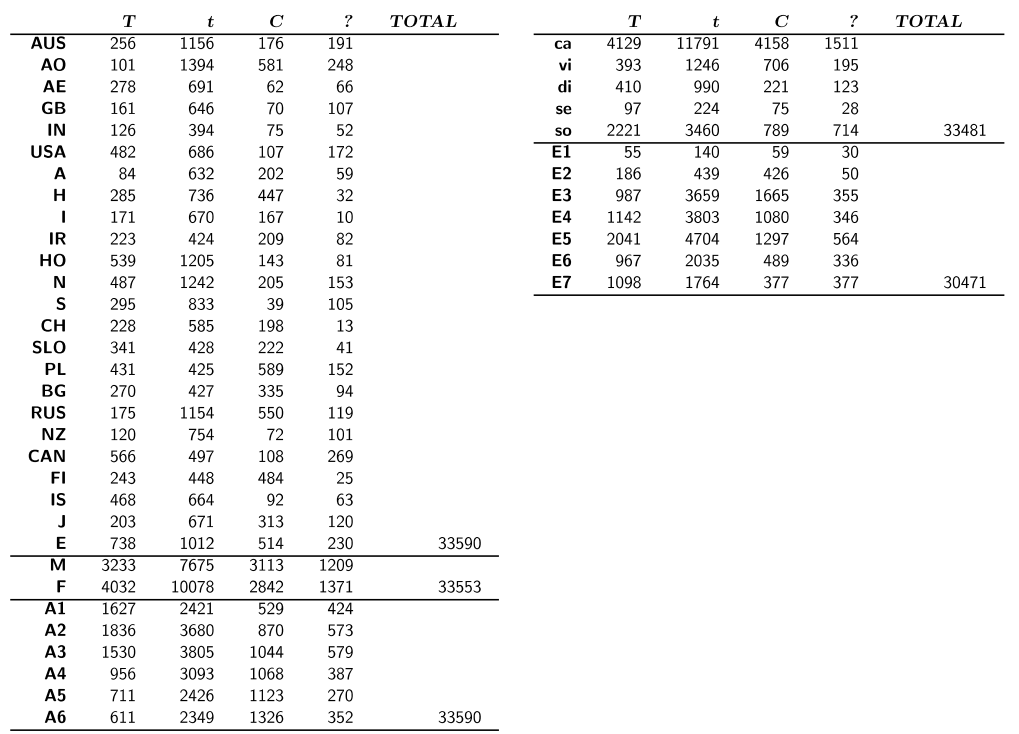
\includegraphics[width=\textwidth]{assets/tablas_apiladas.png}
    \end{figure}
    
    Podemos ver que, si quisiesemos representar el cruce de todas las variables tendríamos $24\cdot2\cdot6\cdot5\cdot7=10080$ categorías frente a las $24+2+6+5+7=44$ que estamos representando ahora.
\end{itemize}

\begin{wrapfigure}{l}{0.5\textwidth}
    \centering
    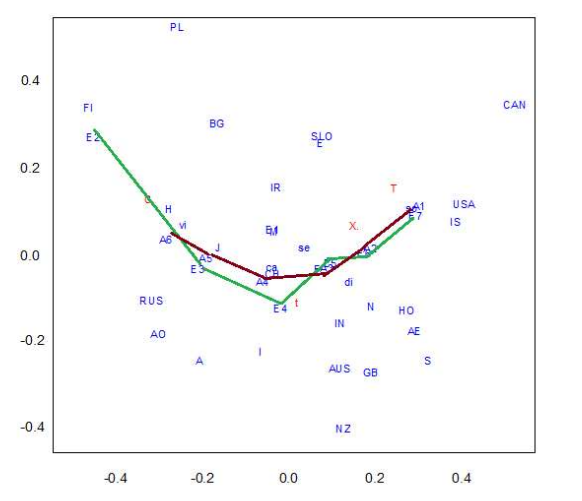
\includegraphics[width=0.5\textwidth]{assets/resultados_concatenadas.png}
\end{wrapfigure}

\noindent Con dos autovalores alcanzamos un 91.2\% de inercia explicada. La interpretación del primer eje que recoge el 63.4\% parece bastante clara. La del segundo es menos directa. Países en la parte alta tienen opiniones más polarizadas y los de abajo más frecuencia en las opiniones intermedias. 

\vspace*{5mm}

\noindent Se puede comprobar además que, si no hay datos ausentes, la inercia de la tabla concatenada es el promedio de las inercias de cada una de las tablas que se han agrupado.

\clearpage

\begin{itemize}
    \item Llamamos $T$ a la tabla completa y $T_1,\dots,T_s$ a las tablas que se agrupan.
    \item $\chi^2_T=\sum_{i=1}^s\chi^2_{T_i}$
    \item Por tanto la inercia total será
    \[
        \text{inercia}(T)=\frac{1}{s}\sum_{i=1}^s\text{inercia}(T_i)
    \]
    \item Tambien se pueden realizar concatenaciones por columnas
    \item \textbf{Análisis de correspondencias múltiples:} El caso en el que se tratan simultaneamente más de dos variables categóricas se denomina análisis de correspondencias múltiples (ACM).
    \item Se tienen $n$ individuos sobre $p$ variables categóricas.
    \item $j_q$ $\forall q=1,\dots,p$ es el número de categorías para la variable $q$.
    \item $J=\sum_{q=1}^p=j_q$.
    \item Los datos vienen representados en una matriz $R=(r_{iq})$ de dimensiones $n\times p$ denominada tabla de modalidades.
    \item El elemento $(i,q)$ contiene la categoría dada por el individuo $i$ en la variable $q$.
    \item Para analizar los datos se construye la matriz binaria (o tabla disyuntiva completa) $Z$ de dimensiones $n\times J$.
    \item $Z=[Z_1,\dots|Z_p]$ donde $Z_q=(z^q_{ij})$ $\forall q=1,\dots,p$ que es una matriz de dimensiones $n\times j_q$ en la que $z^q_{ij}=1$ si la respuesta del individuo $i$ para la variable $q$ ha sido la modalidad $j$ de dicha variable, o 0 en caso contrario.
    \item La \textbf{primera opción} para efectuar un ACM es hacer un AC sobre la matriz binaria $Z$.
    \item $\chi^2_{Z_q}=\sum_{i=1}^{j_q}n(j_q-1)$
    \item $\text{inercia}(Z)=\frac{1}{p}\sum_{q=1}^p\text{inercia}(Z_q)$
    \item Por tanto
    \[
        \text{inercia}(Z)=\frac{1}{p}\sum_{q=1}^p\frac{n(j_q-1)}{n}=\frac{J-p}{p}
    \]
    \newpage
    \item La \textbf{segunda opción} para efectuar un ACM es utilizar la matriz de Burt, que se define como $B=Z'Z$ y tendrá dimensiones $J\times J$ que tiene la forma
    \[
        \begin{bmatrix}
            D_1     & F_{12}  & \cdots & F_{1p} \\
            F'_{12} & D_2     & \cdots & F_{2p} \\
            \vdots  & \vdots  & \ddots & \vdots \\
            F'_{1p} & F'_{2p} & \cdots & D_p
        \end{bmatrix}
    \]

    donde $D_q$ es una matriz diagonal que contiene la distribución marginal de la variable $q$ y $F_{qr}$ es la tabla de contingencia de las variables $q$ y $r$.
    \item Los autovalores obtenidos del análisis de $B$ serán el cuadrado de los autovalores obtenidos con la matriz binaria $Z$
    \item La inercia total es igual al promedio de las inercias de las $p\times p$ submatrices que la componen, y además, la inercia de las matrices diagonales $D_q$ es igual a $j_q-1$.
    \item Las coordenadas factoriales son un reescalado de las obtenidas a partir de la tabla binaria $\varphi_{B,\alpha}(j)=\sqrt{\lambda_{Z,\alpha}}\varphi_{Z,\alpha}(j)$
    \item Los porcentajes de inercia explicados por el análisis de Burt siempre serán superiores a los obtenidos con el otro método.
    \begin{table}[h!]
        \centering
        \resizebox{\textwidth}{!}{
    
        \begin{tabular}[width=\textwidth]{c|cccc|cccc|cccc|cccc|}       
                 & Q1.1 & Q1.2 & Q1.3 & Q1.4 & Q2.1 & Q2.2 & Q2.3 & Q2.4 & Q3.1 & Q3.2 & Q3.3 & Q3.4 & Q4.1 & Q4.2 & Q4.3 & Q4.4 \\
            \hline
            Q1:1 & 2501 & 0    & 0    & 0    & 172  & 1107 & 1131 & 91   & 355  & 1710 & 345  & 91   & 1766 & 538  & 40   & 157  \\
            Q1:2 & 0    & 476  & 0    & 0    & 7    & 129  & 335  & 5    & 16   & 261  & 181  & 18   & 128  & 293  & 17   & 38   \\
            Q1:3 & 0    & 0    & 79   & 0    & 1    & 6    & 72   & 0    & 1    & 17   & 61   & 0    & 14   & 21   & 38   & 6    \\
            Q1:4 & 0    & 0    & 0    & 362  & 1    & 57   & 108  & 196  & 7    & 96   & 205  & 4    & 45   & 45   & 2    & 264  \\
            \hline
            Q2:1 & 172  & 7    & 1    & 1    & 181  & 0    & 0    & 0    & 2    & 165  & 15   & 0    & 0    & 0    & 0    & 1    \\
            Q2:2 & 1107 & 129  & 6    & 57   & 0    & 127  & 0    & 0    & 219  & 997  & 61   & 22   & 972  & 239  & 13   & 75   \\
            Q2:3 & 1131 & 335  & 72   & 108  & 0    & 0    & 1646 & 0    & 24   & 989  & 573  & 60   & 760  & 616  & 84   & 186  \\
            Q2:4 & 91   & 5    & 0    & 196  & 0    & 0    & 0    & 292  & 59   & 4    & 229  & 62   & 60   & 30   & 0    & 234  \\
            \hline
            Q3:1 & 355  & 16   & 1    & 127  & 219  & 24   & 9    & 379  & 642  & 0    & 0    & 0    & 1    & 1    & 1    & 4    \\
            Q3:2 & 1710 & 261  & 17   & 96   & 48   & 997  & 989  & 50   & 0    & 2084 & 0    & 0    & 1348 & 567  & 23   & 146  \\
            Q3:3 & 345  & 181  & 61   & 55   & 4    & 61   & 573  & 4    & 0    & 0    & 313  & 0    & 202  & 286  & 73   & 81   \\
            Q3:4 & 91   & 18   & 0    & 204  & 2    & 22   & 60   & 0    & 0    & 0    & 0    & 49   & 30   & 0    & 0    & 234  \\
            \hline
            Q4:1 & 1766 & 128  & 14   & 51   & 165  & 972  & 760  & 62   & 360  & 1348 & 202  & 49   & 1959 & 0    & 0    & 0    \\
            Q4:2 & 538  & 293  & 21   & 45   & 15   & 239  & 616  & 27   & 14   & 567  & 286  & 30   & 0    & 897  & 0    & 0    \\
            Q4:3 & 40   & 17   & 38   & 2    & 0    & 1    & 0    & 0    & 23   & 0    & 0    & 0    & 0    & 0    & 97   & 0    \\
            Q4:4 & 157  & 38   & 6    & 264  & 1    & 75   & 186  & 203  & 4    & 146  & 81   & 234  & 0    & 0    & 0    & 465  \\
            \hline
        \end{tabular}
        }
        \caption{Ejemplo de tabla de Burt}
    \end{table}
    \item Corrección de los autovalores:
    \[
        \lambda^{\text{adj}}_\alpha=\left(\frac{p}{p-1}\right)^2\left(\sqrt{\lambda^B_\alpha}-\frac{1}{p}\right)^2
    \]
    \item En la Corrección de Benzerí se calculan los porcentajes de inercia correspondiente a cada eje dividiendo por la suma de los autovalores corregidos.
    \item En la Corrección de Greenacre para calcular los porcentajes se divide por la inercia total descontando la de las tablas diagonales. 
    
    Se puede calcular como $\frac{p}{p-1}\left(\text{inercia}(B)-\frac{J-p}{p^2}\right)$.
    \begin{figure}[ht]
        \centering
        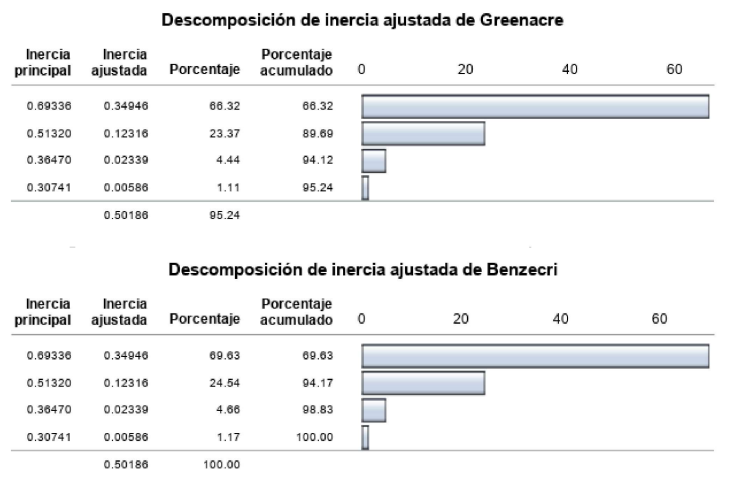
\includegraphics[width=\textwidth]{assets/correcciones_inercia.png}
    \end{figure}
\end{itemize}
